\chapter{Исследовательский раздел}
В данном разделе приведены технические характеристики устройства, на
котором проводилось измерение времени работы программного обеспечения, а
также результаты замеров времени.


\section{Технические характеристики}

Технические характеристики оборудования, на котором проводилось измерение:
\begin{itemize}
    \item операционная система --- Linux;
    \item процессор --- AMD Ryzen 7 5800H;
    \item ОЗУ --- 16 Гб;
\end{itemize}


\section{Цель эксперимента}

Целью эксперимента является сравнение скорости отрисовки кадра
в зависимости от количества граней на сцене и присутствии источника света
модифицированным алгоритмом Z-буфер.

\section{Результаты эксперимента}


В каждом эксперименте создается полотно сцены некоторого размера без объектов,
расположенных на ней. Для каждого такого замера времени позиция наблюдателя
и источника света находятся относительно замеряемой сцены в одном и той же
позиции. Эксперименты проводились 20 раз и усреднялись. На сцене находился
только 1 источник света. На рисунке~\ref{fig:inc-img-science} и на таблице~\ref{tbl:log1}
представлена зависимость времени отрисовки кадра от количества граней на сцене.

\begin{table}[h]
 \begin{center}
  \begin{threeparttable}
  \captionsetup{justification=raggedright,singlelinecheck=off}
  \caption{Зависимость времени отрисовки кадра от количества граней на сцене}
  \label{tbl:log1}
                    \begin{tabular}{|l|l|l|}
                        \hline
                        Количество граней & С иточником света, сек. & Без источника света, сек.\\
                        \hline
                            12 & 0.4 & 0.34 \\ \hline
                            48 & 1.25 & 0.41 \\ \hline
                            108 & 1.45 & 0.42 \\ \hline
                            192 & 1.7 & 0.46 \\ \hline
                            300 & 1.76 & 0.48 \\ \hline
                            432 & 1.91 & 0.49 \\ \hline
                            588 & 2.13 & 0.5 \\ \hline
                            768 & 2.34 & 0.54 \\ \hline
                            972 & 2.41 & 0.57 \\ \hline
                            1200 & 2.55 & 0.59 \\ \hline
                    \end{tabular}
  \end{threeparttable}
    \end{center}
\end{table}

\begin{figure}[htpb]
    \centering
    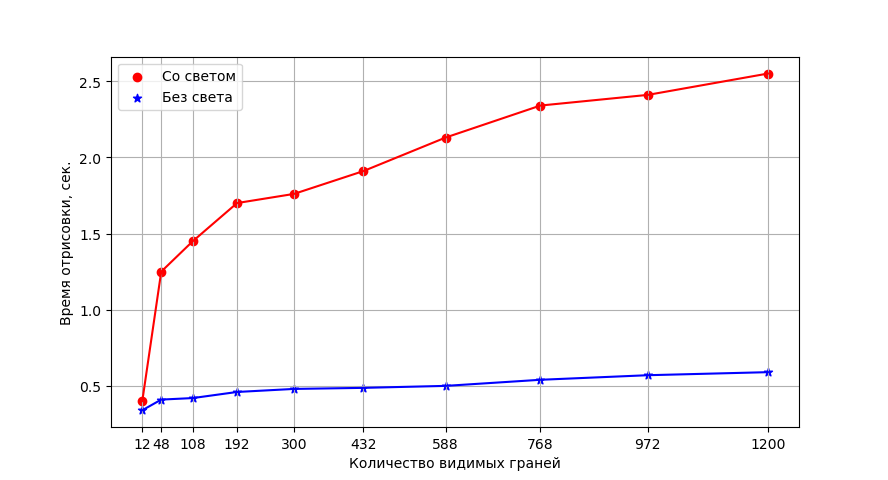
\includegraphics[width=0.7\textwidth]{inc/img/research}
    \caption{Зависимость времени отрисовки кадра от количества граней на сцене}
    \label{fig:inc-img-science}
\end{figure}

%\includeimage
%{research}
%{f}
%{h}
%{0.9\textwidth}
%{Зависимость времени отрисовки кадра от количества граней на сцене}

\clearpage


\section{Вывод}

В данном разделе были приведены технические характеристики устройства,
на котором проводилось измерение времени работы программного обеспечения, а
также результаты замеров времени.

Без учета освещенности алгоритм Z-буфер работает быстрее, чем с учетом освещенности.
Это связано с тем, что для каждого источника света необходимо проинициализировать
и заполнить теневой Z-буфер, а потом для каждого пикселя при растеризации
грани выполнять преобразование координат в координаты в теневом Z-буфере для
определения теней.


